\section{System Overview}
%\section{System Framework}
\label{sec-system}



Figure \ref{fig:framework} shows the framework of \oursystem. It consists of two main components, \ie \emph{Storage} and \emph{Query Engine}.
Below the storage component is a {\em Query-Independent Ranking} module that enriches the data with those pre-computed query-independent ranking scores. Note that there is another {\em Query-Dependent Ranking} module inside the query engine. Finally, two function modules on top present the analysis  to users based on the retrieved results. We next detail our system.

\subsection{Schema Design} \label{subsec:schema}

Graph database Neo4j is adopted for storage in \oursystem. As such, we need to design a schema that abstracts the entities and linked structures (\eg citation, authored-by).
% schema design rationaile
We follow two principles for schema design: (a) nodes for entities and relationships for linked structures, and (b) trading space for query efficiency if affordable and possible.

%reducing fine-grained relationship names while increase generic relationships qualified with property appropriately.

The schema is presented in Fig.~\ref{fig:schema}, where texts nears nodes and relationships represent properties of entities and linked structures, respectively.
It contains seven basic types of nodes including {\em Paper}, {\em Author}, {\em Affiliation}, {\em Venue}, {\em FOS} (field of study), {\em ConIns} (conference instance in each year) and {\em Year}.
In addition, it further incorporates an artificial type of nodes, \ie {\em PAA} representing paper-author-affiliation tuples. Here we trade extra space cost for query efficiency, \ie an author and her/his affiliation can be retrieved in one query.
%
Our schema also forms a total of nine types of relationships, one of which, \ie {\em :VenueScore}, has a weight property {\em score} and the rest are unweighted.
As another space-efficiency trade-off, those {\em Paper} nodes also use extra space on properties to maintain conference ID, journal ID and year.



\begin{figure}
\centering
\subfigure[{\scriptsize Framework}]{\label{fig:framework}
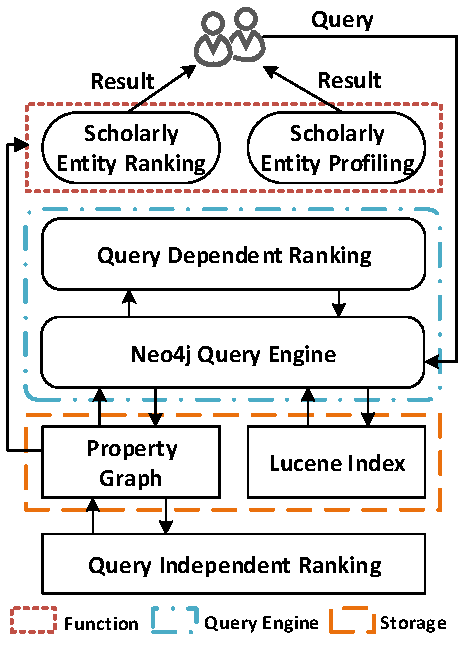
\includegraphics[width=0.45\columnwidth]{systemFrame.pdf}}
%\hspace{3ex}
\subfigure[{\scriptsize Neo4j schema}]{\label{fig:schema}
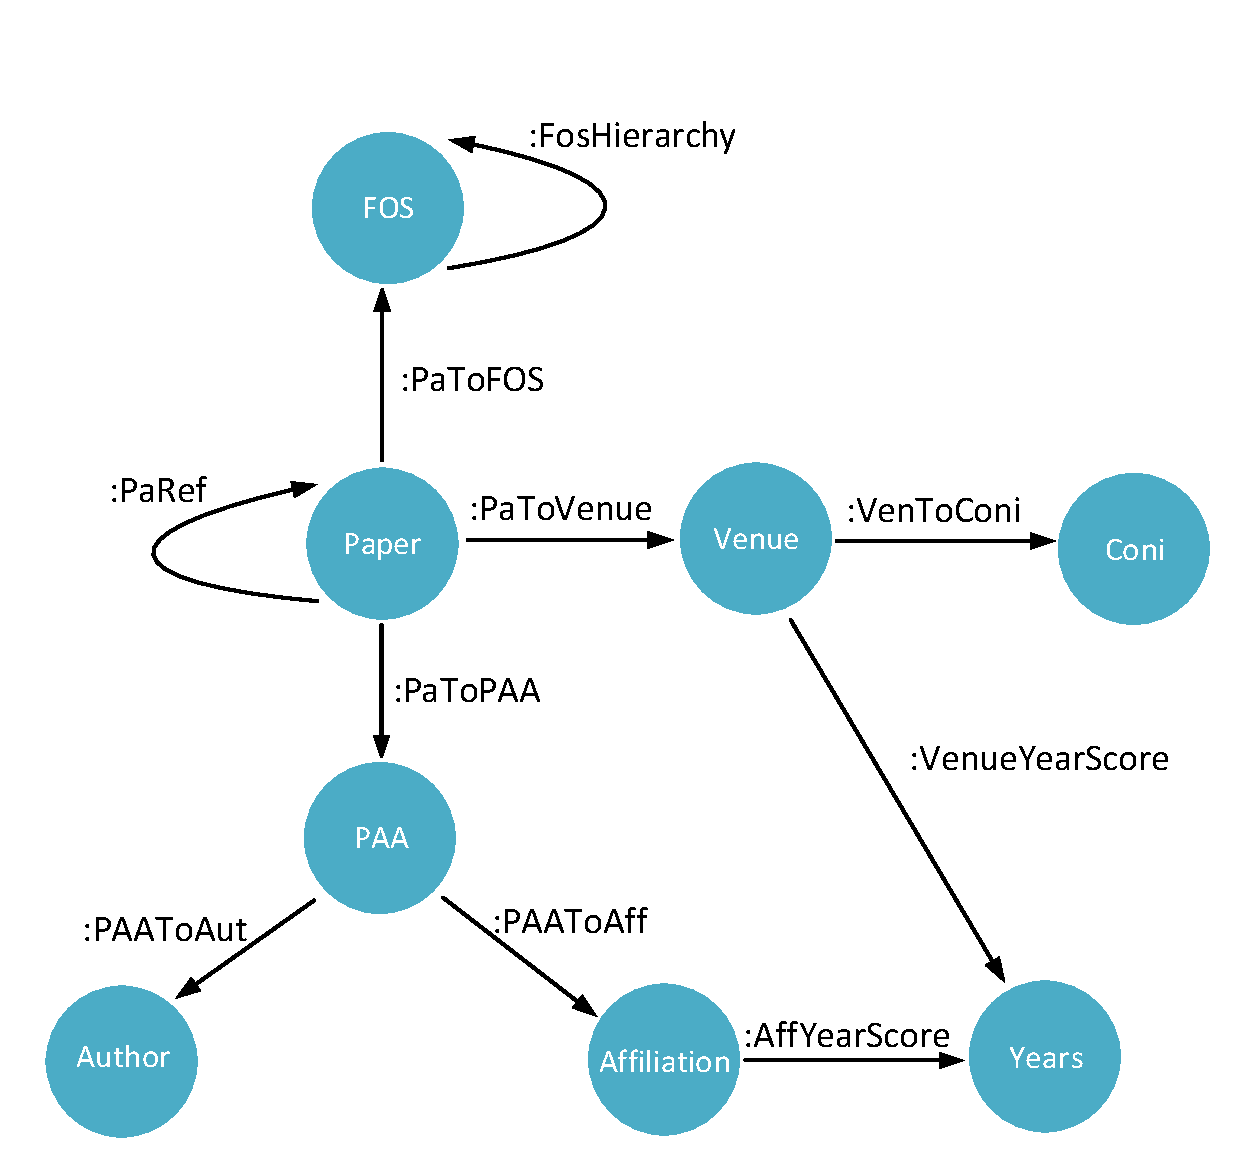
\includegraphics[width=0.5\columnwidth]{neo4jSchema.pdf}}
\vspace{-1ex}
\caption{System design of \oursystem}
\label{fig:system}
%\vspace{-2ex}
\end{figure}


\subsection{Graph Storage} \label{subsec:storage}


Based on the above schema, we maintain our scholarly data, \ie MAG~\cite{sinha2015overview}, as a huge property graph with more than 1.03 billion nodes and 1.93 billion relationships. We further clarify our graph storage with the following.


First, based on the original scholarly data, the {\em Query-Independent Ranking} module pre-computes those query-independent ranking scores, \ie numbers of citations of papers, importance scores of papers, authors, venues and affiliations~\cite{ma2018query}. These scores are assigned as properties to the corresponding nodes.
Note that iteratively accessing the linked entities is the most essential operation in the pre-computation. And it is much more convenient with graph storage.
Moreover, both citation numbers and importance scores support incremental computation~\cite{ma2018query} and are easier to dynamically maintain once the property graph gets updated.


Second, to facilitate query processing on the billion-scale property graph, Lucene index is utilized for initial entity lookups. Specifically, we create fulltext indices for paper titles and affiliation names. These enable to efficiently find papers and affiliations whose titles and names contain a specific keyword. Besides, we also create schema indices for the entire author and venue names. %for efficient initial entity lookup.


%\begin{figure}
%\centering
%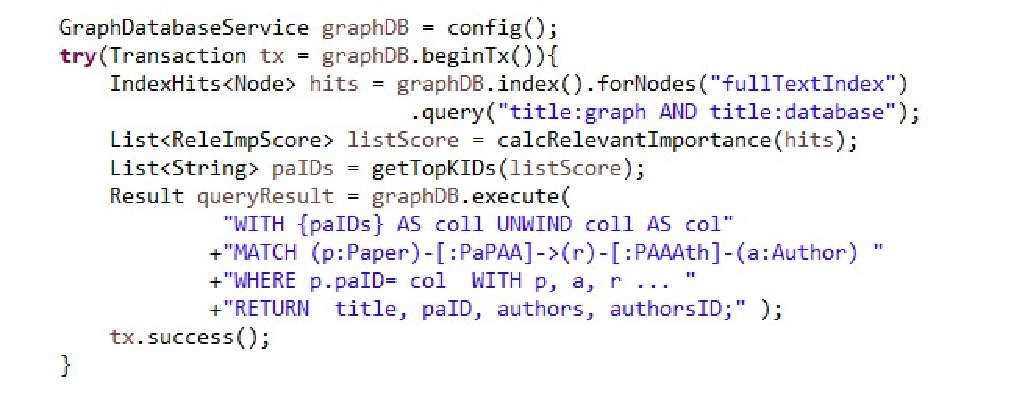
\includegraphics[width=\columnwidth]{queryProcess.pdf}
%\vspace{-3ex}
%\caption{An example workflow of the query engine}
%\label{fig:queryProcess}
%%\vspace{-2ex}
%\end{figure}

\subsection{Graph Query Engine} \label{subsec:qe}
\oursystem supports a variety of graph queries on the property graph. And the {\em Query Engine} is responsible for processing this set of queries. When a query is issued, {\em Neo4j Query Engine} first translates it into a cypher with proper parsing and semantic analysis.
Note that, when applicable, the cypher also includes the entity IDs returned from the Lucene index. Rankings given by the {\em Query-Dependent Ranking} module, \ie relevance and relevant importance-based rankings, may also be included in the cypher if needed. Based on the final cypher, an optimized query plan is generated and processed on the property graph.

%Figure~\ref{fig:queryProcess} 

Table~\ref{tab-workflow} gives an example workflow of the query engine that users want to retrieve the top scholarly articles about ``graph database"  ranked by relevant importance. The fulltext index is firstly hit to get the related paper IDs on ``graph database'' (lines 3--4). The {\em Query-Dependent Ranking} module then calculates the relevant importance scores of those related papers and the top-k paper IDs are further identified (lines 5--6). Based on the complete cypher (lines 7--12)., the {\em Neo4j Query Engine} finally generates the query plan, executes it on the property graph and gets the results.

\subsection{Function Modules}
Finally, the two function modules on top collect the scholarly entities ranked and returned from the back-end, and present some (visual) analysis to users. Moreover specifically, \oursystem utilizes RESTful APIs  and Echarts\footnote{http://echarts.baidu.com/} to display the scholarly ranking and profiling. Detailed demonstrations are available in next section.


% visualization do what ?
% restful API
% scenarios, Query and Ranking Scholarly Entity, Author Profiling.
%Based on the graph storage, scholarly data was managed and processed in the system back-end. \oursystem collects user querys, dispatch to query engine and the results are then presented by visualizer using RESTful API. We employ Echarts (http://echarts.baidu.com/) to display scholarly article analysis and author profiling, detailed demonstrations are accessed in next section.
% function implement in back-end, echarts js  using RESTful API. demonstrate xxx in the next section.


%With scholarly data management and processing in the system back-end, the visualizer of \oursystem collects user queries through user interfaces. The queries are to the query engine and the returned results are then presented by visualizer. We will demonstrate some scholarly analysis scenarios in the next Section.


\begin{table}[t!]
%\begin{center}
\caption{An example workflow of the query engine}
\label{tab-workflow}
\begin{scriptsize}
\begin{tabular}{ l}
\hline
{An example workflow of the query engine} \\
\hline
1. GraphDatabaseService graphDB = new GraphDatabaseFactory()... ; \\
2.  \hspace{0ex}  try(Transaction tx = graphDB.beginTx()) \{ \\
3.  \hspace{4ex} 	IndexHits $\langle$ Node$\rangle$ hits = db.index().forNodes(``fullTextIndex") \\
4.  \hspace{8ex}   .query("title: graph AND title:database"); \\
5.  \hspace{4ex} 	List$\langle$ ReleImpScore$\rangle$ listScore = calcReleImpo(hits, ``graph database"); \\
6.  \hspace{4ex} 	List$\langle$ String$\rangle$  paIDs = getTopKIDs(listScore); \\
7.  \hspace{4ex}    Result result = graphDB.execute(`` \\
8.  \hspace{8ex}		WITH \{paIDs\} AS IDs UNWIND IDs AS perID \\
9.  \hspace{8ex}		MATCH (p:Paper)-[:PaToPAA]-$>$(r)-[:PAAToAut]-(a:Author)\\
10.	\hspace{7ex}		WHERE p.paID= perID \\
11. \hspace{7ex}        WITH p.title,  COLLECT(a.auName), SIZE(()-[:PaRef]-$>$(p)) AS cite, r \\
12.	\hspace{7ex}		RETURN  paID, title, authors, cite ... ");\\
13.	\hspace{4ex}	    tx.success();\\
14. \hspace{2ex}  \} \\
\hline
\end{tabular} \\ %\vspace{.5ex}
\end{scriptsize}
%\end{center}
\end{table}

